\section{深度学习介绍}

\subsection{传统机器学习方法与局限性}

在之前的50年左右,传统的模式识别模型用手工定义的特征进行特征提取,通过对数据的分析选取可训分类器进行模型构建。 最近10年,借助现代计算机计算能力的提高和大数据量的爆发,神经网络方法得以重新广泛应用,在很多领域都达到非常好的效果, 我们称这种利用大规模网络进行模式识别方法为深度学习(Deep Learning), 也叫End-To-End Learning。不同于传统模型采用固定特征,或者固定kernel(核函数)进行样本度量; 深度学习采用可训特征(或可训的kernel), 然后将特征作为可训练的分类器输入, 进行训练, 如表\ref{Tab:dl_overview_compare}。

\begin{table}[ht]
\centering
  \begin{tabular}{|c||c|c|c|}
  \hline
   & 特征 & 分类器 & 特点\\
  \hline\hline
   传统方法 & 人工定义的特征 & 简单可训练分类器 & 特征设计费时,需强业务背景\\
  \hline
  深度学习 & 训练特征提取模型 & 复杂可训练分类器 & End-to-End learning,feature易操作\\
  \hline
  \end{tabular}
  \caption{深度学习与传统模式识别方法}
  \centering \label{Tab:dl_overview_compare}
\end{table}

历史上,第一个有学习功能的机器为1960年提出的Perceptron\cite{rosenblatt1960perceptron},也是神经网络的一个基本单元。 Perceptron是一个简单特征提取器上加载的一个线性分类器: 


\begin{equation}
\label{Eq:Perceptron}
y=sign(\sum_{i=1}^N{w_iF_i(x)}+b)
\end{equation}


其中$x$为数据,$F_i(x)$为x的第i个特征,$w_i$为相应的特征权重参数, b为常参数, $sign$为分类器的非线性函数,对于二类分类,$sign$函数将结果映射到(0,1)。

\begin{figure*}[htb]
  \centering
  % Requires \usepackage{graphicx}
  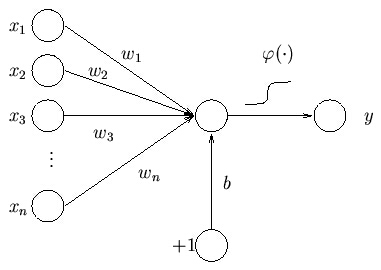
\includegraphics[scale=0.9]{Pictures/CNN/perceptron.jpg}\\
  \caption{Perceptront图例}\label{fig:perceptron}
\end{figure*}

目前最普及的实际应用也用到了线性分类器的一些变种,或者叫模板匹配(template matching)。 但是由于其底层的特征提取器需要反映特定信号的特点, 所以需要由特定领域专家来设置。 比如图像处理领域, 对于不同任务( 图像分类, 图像分割, 图像跟踪等), 所要求的特征就各不相同, 需要针对特定任务定义图像特征。 此外,传统方法也很难设计kernel, 从而不容易表达对距离的度量,仍然以图像来说,最简单的距离度量思路是对应像素相减,但是这显然不能表达图像语义层的相似信息。

为了能使特征更加灵活而且不过多依赖于专家指定的特征, 很多方法提出, 可以先人为定义简单特征, 然后通过无监督学习方法进一步得到中间层特征, 将其输入分类器进行最后分类。
典型的无监督特征学习方法如混合高斯模型\cite{jeong2004image,gray2001gauss,gauvain1992bayesian,reynolds2000speaker,reynolds1995robust, zivkovic2004improved,lee2005effective,yang1999gaussian}, K-Means\cite{liu2007computational,netzer2011reading,coates2011text,dy2004feature,coates2012learning}, 和Sparse Coding\cite{yang2009linear,boureau2008sparse,coates2011importance,coates2011analysis,gao2010local,mairal2010online}。 但这仍然不能解决以下几个问题:

\begin{enumerate}
	\item 建立传统模型代价大\\
	对每个领域,每个任务都需要设计特征。即便有了中间特征层进行无监督的特征选择, 庞大冗余的基础特征的设计也是耗时费力的。 随着工业界对不同任务的需求, 需要建立很多基础特征、 模型, 代价也很大。
	\item 无法很好地利用计算性能\\
	计算机性能的大幅提升本可以用来帮助加速机器学习, 但传统机器学习需要人工定义模型, 从而使模型规模受限,不能很好地利用计算性能和大量数据。 
	
	\item 人工定义特征效果欠佳\\
	目前, 自动学习的特征已经在图像、语音等很多领域强于人工定义的特征。 而且如果需要增加特征维度进行大规模学习就需要再手工定义更多特征, 而不能简单地够自动按比例扩大。
	
\end{enumerate}


\subsection{深度学习方法介绍}

深度学习是近几年来很热的机器学习算法, 在语音识别,计算机视觉,自然语言处理等领域打破了维持了多年的竞赛记录。以最典型的时序模型——语音识别的发展为例, 在1980年代早期, 主要应用Dynamic time Warping (DTW)\cite{juang1984hidden,myers1981comparative,rabiner1978considerations,berndt1994using}, 输入底层特征,通过无监督学习所得中间层特征输入分类器进行分类。 1985年后, \cite{huang1990hidden,rabiner1989tutorial,rabiner1986introduction}提出在中间层用隐马尔科夫模型描述一个序列出现的概率,得到进一步改进。 2010年左右, 使用深度神经网络进行逐层有监督学习达到最佳效果\cite{waibel1989modular,nakamura1989speaker}。


同传统方法的基本方法类似, 深度学习也是从数据分别生成底层特征, 中间层特征, 最后加入高层特征, 输入分类器进行分类, 即学习数据的结构化表示。 其形式化表示为:
\begin{equation}
y=F(W^kF(W^{k-1}F(...F(W^0X)...)))
\label{Eq:dl_formulation}
\end{equation}
其中, W为权重参数,k为层数,$W^iX$为输入X的线性表示, $F$为非线性函数。 深度学习就是优化$y$与groundtruth之间的距离,使之最小化。 从图像角度, 如图\ref{fig:feature_level}所示\cite{zeiler2014visualizing,zeiler2013stochastic},图中(a),(b),(c)分别为自动学得的底层特征,中层特征和高层特征, 其中底层特征学习图像的浅层特征,在所有类别中共享, 如(a)中,学到的特征类似Gabor滤波器所提取的边缘特征\cite{ngiam2010tiled,shi1998gabor}, 从中间层到高层依次学习图像更深层的语义特征, 如有语义的显著图像区域, 高层特征更为稳定,也具有类属性。  从自然语言处理的角度, 初始输入为字符, 从底层向上依次学习单词, 短语, 长句, 文章。

\begin{figure*}[htb]
  \centering
  % Requires \usepackage{graphicx}
  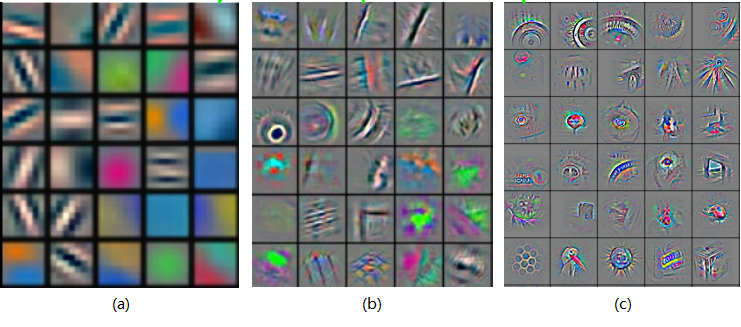
\includegraphics[scale=0.9]{Pictures/CNN/low_mid_high_feature.png}\\
  \caption{各层次feature}\label{fig:feature_level}
\end{figure*}


除了自动学习特征外, 深度学习和传统模型还有一个重要区别就是“深”。 一般来说, 深度结构由多层含参的非线性模型组成, 以形成特征的层次结构。
在\cite{bengio2007scaling,bengio2009learning}中讨论了深度模型的必要性。 浅层结构以现在的kernel machine\cite{scholkopf1999advances}为例, 如Support Vector Machine(SVMs)\cite{boser1992training,cortes1995support}。 这些方法定义特征
为一系列kernel函数连接而成的向量, 在训练数据中进行模板匹配, 如式\ref{Eq:kernel_fea_vec}所示。

\begin{equation}
	\label{Eq:kernel_fea_vec}
	\varphi(x) = [k(x,\mu_1),k(x,\mu_2),...,k(x,\mu_n)]
\end{equation}

式中, $\mu_i$为数据样本的一部分, 即模板样本; $\varphi(x)$为样本$x$的特征。 而后$\varphi(x)$通过线性组合进行分类:


\begin{equation}
	\label{Eq:kernel_predict}
	F(x) = W^T\varphi(x)
\end{equation}

可见, kernel方法就是一个简单的模板匹配层连接一个线性函数层, 由于方法中模板都是从原始训练数据中提取而得, 所以kernel machine的第一层
可视作一种简单的无监督方法, 只有式\ref{Eq:kernel_predict}中参数$W$的学习为有监督部分,没有涉及特征的层次结构, 因此不是深度模型。 同样,只有一个隐层的模型(如multilayer perceptron)也不算深度模型。 又如分类回归树(Classification and Regression Tree, CART), 其中所有决策都是在输入空间定义的, 同样没有根据特征的层次结构进行学习, 因此也不属于深度模型。 虽然有一些理论保证浅层结构可以很好地拟合任何复杂函数, 它们却无法保证特征的高效表征。 而深度模型可以从根本上通过简单设置网络结构更有效地表示特定函数。 最典型的深度结构就是有多个隐层的神经网络, 其中每个隐层节点之间的连接权重(如图\ref{fig:perceptron}中的$w_i$)都是通过有监督学习而来的, 因此可以很好地表征数据属性。



\begin{figure*}[htb]
  \centering
  % Requires \usepackage{graphicx}
  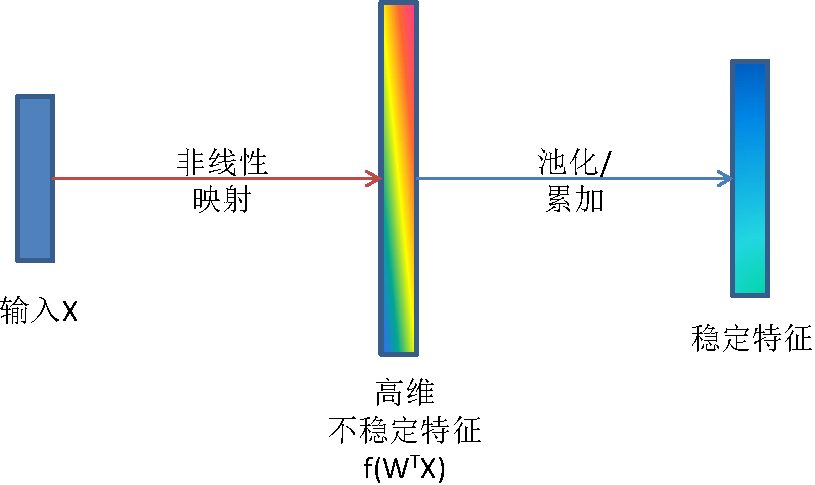
\includegraphics[scale=0.8]{Pictures/CNN/invariant-feature-crop.pdf}\\
  \caption{稳定特征生成方法}\label{fig:invariant_feature_learning}
\end{figure*}


神经网络在1940年代就开始了相关研究\citep{mcculloch1943logical,hebb1949organization}
, 但早期提出的神经网络多为线性回归的变种, 没有很大突破。 1960年代,受神经科学的启发, 神经网络也随之发展。 当时神经科学在猫的视觉皮层发现了简单细胞和复杂细胞, 简单细胞对特定视觉输入(如边缘的方向)敏感, 会做出一定响应; 而复杂细胞相对简单细胞表现出更为鲁棒的响应, 即不受空间变化的影响。 这一特性使得神经网络向更深层发展, 也就是“深”的结构。 1965年, \cite{}提出了第一个深度学习模型——Group Method of Data Handling (GMDH), 它通过回归方法进行网络训练, 再通过决策正则化去掉多余节点。 直到现在仍有很多应用以GMDH为基本框架, 如\cite{}Ikeda et al., 1976; Farlow, 1984; Madala and Ivakhnenko, 1994;
Ivakhnenko, 1995; Kondo, 1998; Kord´ık et al., 2003; Witczak et al., 2006; Kondo and Ueno, 2008。 1979年, \cite{}第一次在Neocognitron中引入了卷积神经网络的概念。 其结构和现在我们用到的前向卷积神经网络比较相似, 也是基于梯度的深度学习方法。 只是, Neocognitron通过无监督的方法得到网络参数, 而不同于现在的有监督误差反传方法。 



由于90年代计算资源和数据量受限, 当隐层层数大于2的时候深度网络训练困难\cite{tesauro1992practical}, 所以之前神经网络的研究工作主要集中于浅层结构。 随着现在数据量的爆发, 神经网络的研究变得重新热门起来。 其基本思想是学习具有不变性的特征, 即,将输入数据映射到一个非线性的高维空间,使数据变得可分。 如\ref{fig:invariant_feature_learning}所示,输入经过非线性函数的映射到高维特征, 使数据变得可分, 但是这样的高维特征可能由于训练数据间差异导致不稳定,所以将高维数据中相似语义信息的成分通过池化(pooling)或累加等方法整合到一起, 形成稳定特征。





\subsection{深度神经网络结构与训练}

\begin{list}{•}

\item 网络结构



从网络结构来分, 神经网络有前向网络(包括multilayer neural nets\cite{kuurkova1992kolmogorov,
hornik1989multilayer,hornik1991approximation}和 convolutional nets \cite{lecun1995convolutional,krizhevsky2012imagenet},), 回馈网络(包括 stacked sparse coding\cite{yu2011learning}, deconvolutional nets\cite{zeiler2010deconvolutional})和双向网络(包括 deep boltzmann machines\cite{salakhutdinov2009deep,
srivastava2012multimodal,goodfellow2013multi}, stacked auto-encoder\cite{gehring2013extracting,vincent2010stacked,vincent2008extracting})三类\cite{lecun2013deep}。 目前, 前向网络使用最广, 如图\ref{fig:feed_forward}所示为一个前向网络的示意图。 




\begin{figure*}[htb]
  \centering
  % Requires \usepackage{graphicx}
  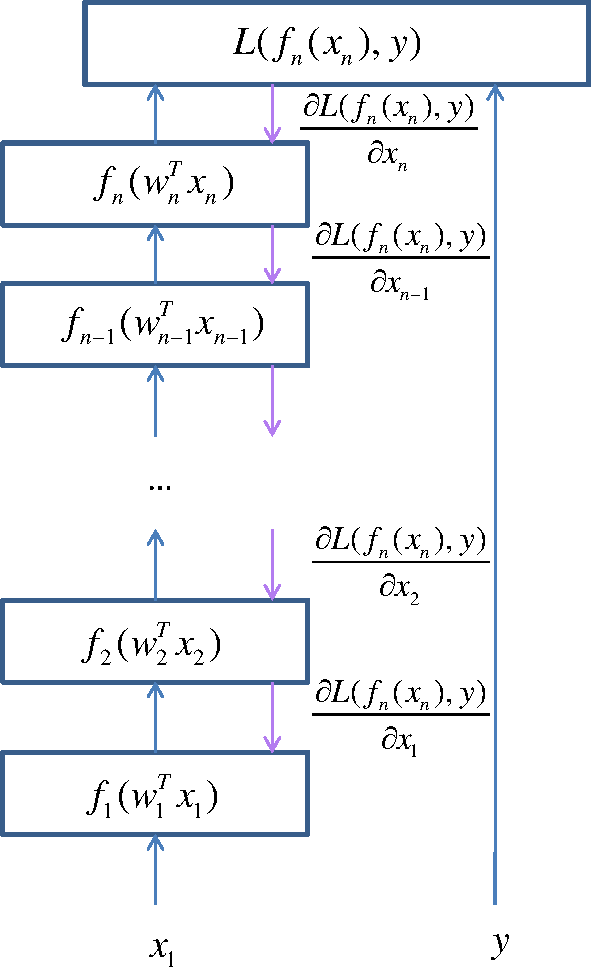
\includegraphics[scale=0.9]{Pictures/CNN/feed-forward-crop.pdf}\\
  \caption{前向网络的网络结构}\label{fig:feed_forward}
\end{figure*}



其中, $x_i$表示第i层的输入, 整个网络的输入为$x_1$; $w_i$表示第i层的参数, $w_i^Tx_i$得到$x_i$的线性组合; $f$为非线性函数, 每一层通过非线性函数将输入数据映射到下一层, 如图中蓝色箭头所示。 经过每一层非线性映射$f_i$的刀下一层输入,即
\begin{equation}
 x_i = f_{i-1}(w_{i-1}^Tx_{i-1})
\end{equation}

给定$x_1$对应的样本label$y$,我们的目标函数为$L(f_n(x_n),y)$, 其中$L$为损失函数。 常见的损失函数有平方损失, 指数损失, 对数损失等。 




\item 训练方法


我们希望最小化损失函数的值, 可以用误差反传算法(back-propagation algorithm)\cite{hecht1989theory,goh1995back}对每个$x_i$的求导结果更新参数$w$,如图中向下的紫色箭头所示, 可通过将误差逐层传递训练网络。

\begin{equation}
\frac{\partial L}{\partial x_{n-1}} = 
\frac{\partial L}{\partial x_n}
\frac{\partial f_{n-1}(w_{n-1}^Tx_{n-1})}{\partial x_{n-1}}
\end{equation}




\end{list}




其中卷积神经网络属于前向网络, 广泛应用于图像识别。 我们将在第\ref{sec:CNN}节中介绍卷积神经网络的结构与训练过程, 在第\ref{sec:cnn_configure}节中介绍我们的数据与网络配置, 最后在第\ref{sec:cnn_experiment}中给出实验结果。


\section{卷积神经网络}\label{sec:CNN}


\subsection{Perceptron}

\subsection{CNN网络结构}


\section{ConvP300Net}\label{sec:cnn_configure}

\subsection{任务描述}

\subsection{网络结构}

\section{实验结果}\label{sec:cnn_experiment}













